\documentclass[border=3pt]{standalone}
% Preâmbulo compartilhado pelos diagramas TikZ da aula 13 (SLAM com EKF)
\usepackage[T1]{fontenc}
\usepackage[utf8]{inputenc}
\usepackage{lmodern}
\usepackage{amsmath}
\usepackage{xcolor}
\usepackage{tikz}
\usetikzlibrary{arrows.meta,angles,quotes,decorations.pathmorphing,decorations.pathreplacing,calc,
                positioning,shapes.geometric,shapes.misc,backgrounds,fit,
                math}

% Paleta (mesma dos SVGs originais)
\definecolor{dblue}{HTML}{2A5B8C}
\definecolor{dorange}{HTML}{B3541E}
\definecolor{dgreen}{HTML}{4A7C59}
\definecolor{dred}{HTML}{9C4B4B}
\definecolor{dcream}{HTML}{F4F1EA}
\definecolor{dshade}{HTML}{DDD7C9}

% Função gaussiana (não normalizada por padrão de escala visual)
\pgfmathdeclarefunction{gauss}{3}{%
  \pgfmathparse{1/(#3*sqrt(2*pi))*exp(-((#1-#2)^2)/(2*#3^2))}%
}

% Estilos comuns (prefixo d... para não colidir com chaves internas do pgf)
\tikzset{
  >={Stealth[length=2mm]},
  dguide/.style={gray!55, dashed, line width=0.4pt},
  daxis/.style={gray!60, line width=0.7pt, ->},
  dbody/.style={fill=black!3, draw=black!80, line width=1pt},
  dacc/.style={draw=dblue, line width=1pt},
  dlbl/.style={black!55, font=\small},
  dsub/.style={black!45, font=\footnotesize},
  dstate/.style={circle, draw=black!80, fill=dcream, line width=1pt,
                 minimum size=17mm, font=\large, inner sep=1pt},
  dobs/.style={circle, draw=black!80, fill=dshade, line width=1pt,
               minimum size=14mm, font=\large, inner sep=1pt},
  dbox/.style={rounded corners=2pt, draw=black!80, fill=dcream, line width=1pt,
               align=center, inner sep=6pt},
  dop/.style={circle, draw=black!80, fill=white, line width=1pt,
              minimum size=6mm, inner sep=0pt, font=\small},
  dtrans/.style={->, dblue, line width=1pt},
  dmeas/.style={->, dorange, line width=1pt},
  dcurve/.style={line width=1pt, dblue},
  dcurveb/.style={line width=1.4pt, dorange},
}

\begin{document}
\hyphenpenalty=10000 \exhyphenpenalty=10000 \tolerance=9999 \emergencystretch=3em
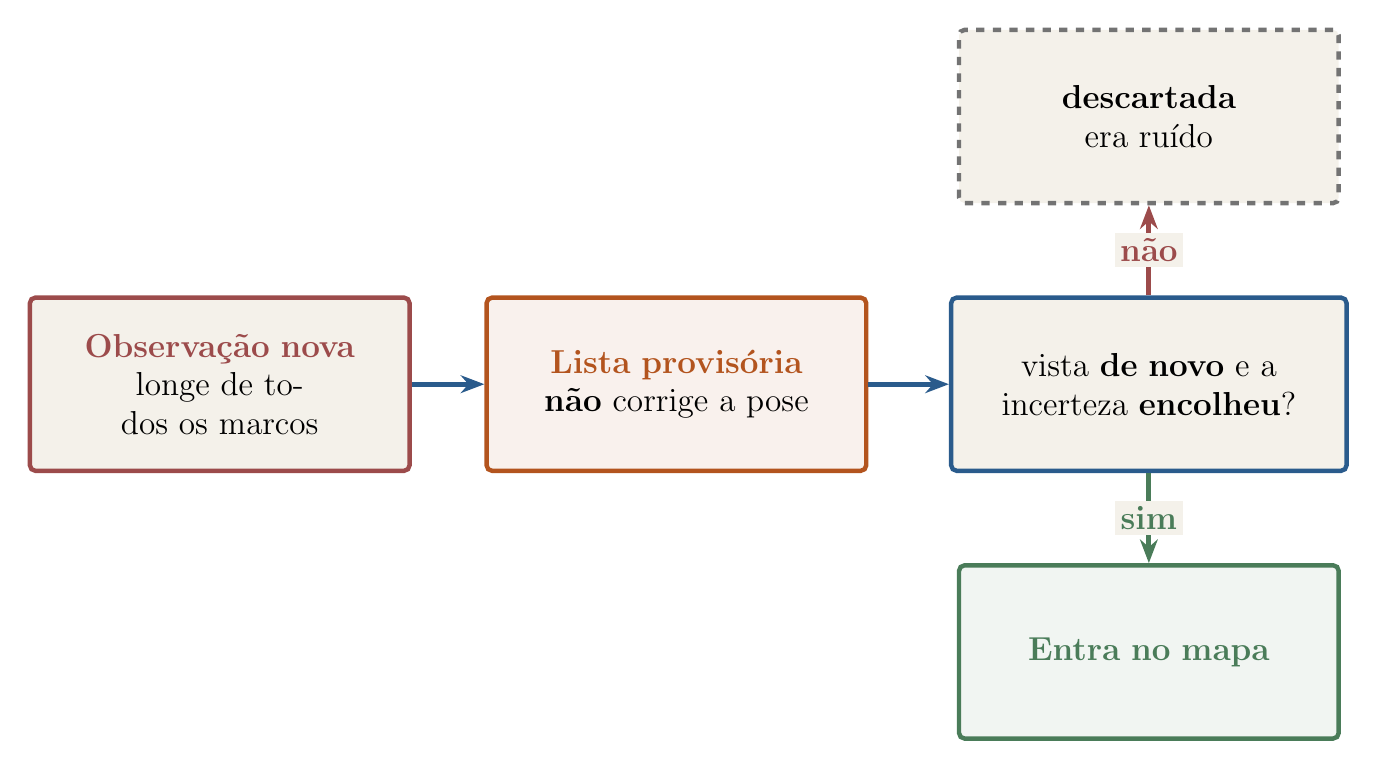
\begin{tikzpicture}[x=1cm,y=1cm]
\tikzset{c/.style={dbox, text width=4.4cm, minimum height=2.2cm, font=\large, line width=1.6pt},
        q/.style={dbox, draw=dblue, text width=4.6cm, minimum height=2.2cm, font=\large, line width=1.6pt},
        a/.style={dtrans, line width=1.9pt, -{Stealth[length=3mm]}},
        l/.style={font=\large\bfseries, fill=dcream, inner sep=2pt}}
\node[c, draw=dred] (n) at (2.4,4.6) {\textbf{\textcolor{dred}{Observação nova}}\\ longe de todos os marcos};
\node[c, draw=dorange, fill=dorange!8] (p) at (8.2,4.6) {\textbf{\textcolor{dorange}{Lista provisória}}\\ \textbf{não} corrige a pose};
\node[q] (d) at (14.2,4.6) {vista \textbf{de novo} e a incerteza \textbf{encolheu}?};
\node[c, draw=dgreen, fill=dgreen!8] (m) at (14.2,1.2) {\textbf{\textcolor{dgreen}{Entra no mapa}}};
\node[c, draw=black!55, dashed] (x) at (14.2,8.0) {\textbf{descartada}\\ era ruído};
\draw[a] (n.east) -- (p.west);
\draw[a] (p.east) -- (d.west);
\draw[a, dgreen] (d.south) -- node[l, text=dgreen] {sim} (m.north);
\draw[a, dred] (d.north) -- node[l, text=dred] {não} (x.south);
\end{tikzpicture}
\end{document}
